\documentclass[conference]{IEEEtran}
\IEEEoverridecommandlockouts

% ==== Fonts & core packages ====
% IEEE推奨のTimes系に近い newtx 系
\usepackage{newtxtext,newtxmath}

\usepackage{graphicx}
\usepackage{amsmath} % amssymb は newtxmath と衝突しやすいので未使用
\usepackage{cite}
\usepackage{tikz}
\usetikzlibrary{arrows.meta,positioning}
\usepackage{xcolor}
\usepackage[hidelinks]{hyperref}

% 図の横幅を安全に抑えるヘルパー
\newcommand{\fitfig}[1]{\resizebox{0.92\linewidth}{!}{#1}}

\title{Educational Perspectives on Complementary FETs (CFET):\\
Evolution Beyond GAA and Open Challenges}

\author{
\IEEEauthorblockN{Shinichi Samizo}
\IEEEauthorblockA{Independent Semiconductor Researcher\\
Project Design Hub, Samizo-AITL\\
\textit{Email:} \href{mailto:shin3t72@gmail.com}{shin3t72@gmail.com}\quad
\textit{GitHub:} \href{https://github.com/Samizo-AITL}{Samizo-AITL}}
}

\begin{document}
\maketitle

\begin{abstract}
This tutorial paper provides an educational overview of emerging
\emph{Complementary FET (CFET)} technology, which vertically stacks nFET and pFET devices beyond Gate-All-Around (GAA) nanosheets.
CFET reframes the CMOS inverter as a \emph{cross-sectional} integration, promising density and delay improvements.
We consolidate structure, electrostatic motivations, layout and delay impacts, fabrication challenges, and modeling limitations, and articulate the pedagogical value of CFET as an open, unresolved technology for semiconductor curricula.
\end{abstract}

\begin{IEEEkeywords}
CFET, GAA, FinFET, nanosheet FET, short-channel effects, scaling, education, tutorial, vertical stacking, PDK.
\end{IEEEkeywords}

% =========================
\section{Introduction}
Scaling has progressed from planar CMOS to FinFET and most recently GAA nanosheet FETs.
Beyond the 2\,nm node, interconnect delay and cell footprint limit further gains despite excellent electrostatics.
CFET stacks nFET and pFET in the vertical dimension so that the cross-section itself constitutes a CMOS inverter, potentially doubling effective standard-cell density while shortening n--p connections.
This paper positions CFET as both a roadmap element and an educational vehicle for device--design co-optimization.

% =========================
\section{Device Evolution: From SCE Relief to Cross-Sectional CMOS}
\label{sec:evo}
\subsection{Planar CMOS and SCE Motivation}
As gate lengths entered the deep sub-100\,nm regime, planar MOSFETs suffered
from short-channel effects (SCE): threshold-voltage roll-off, drain-induced barrier lowering, off-state leakage, and degraded subthreshold slope.
Electrostatic control by a single top gate could no longer effectively pinch off the channel as depletion regions overlapped.

\subsection{FinFET: Three-Sided Gate Control}
FinFETs improved electrostatics by wrapping the gate around \emph{three} sides of a vertical fin.
The stronger gate-to-channel coupling sharpened subthreshold slope, reduced variability, and enabled higher drive per footprint by using multiple fins per device.
However, the tall/narrow fin introduced process and variability trade-offs and left one side of the channel uncontrolled.

\subsection{GAA Nanosheet: Four-Sided Control}
Gate-All-Around (GAA) nanosheet FETs extend control to \emph{four} sides by surrounding suspended sheets (or wires) with the gate.
This architecture further suppresses SCE and variability and allows continued gate-length scaling.
Yet, at advanced nodes the delay/energy bottleneck increasingly shifts from device electrostatics to \emph{wiring}: local interconnect resistance/capacitance (RC) and the lateral footprint of standard cells.

\subsection{CFET: Stacking Complementary Devices}
CFET addresses wiring and density limits by placing nFET and pFET in the \emph{same lateral footprint} and connecting them vertically.
Two immediate educational takeaways are:
(i) effective cell density can approach $\sim 2\times$ by sharing diffusion/gate footprint across polarities; and
(ii) the critical n-to-p connection in inverters and logic stacks shortens, reducing local RC and stage delay.
In short, CFET reframes CMOS as a \emph{cross-sectional inverter} rather than a lateral pair.

\begin{figure}[htbp]
\centering
\fitfig{%
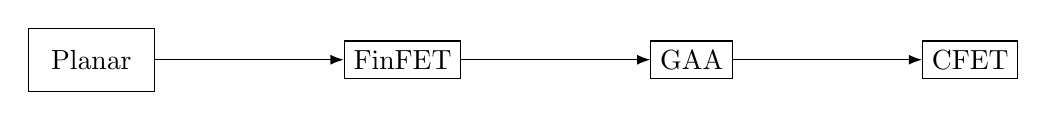
\begin{tikzpicture}[node distance=2.4cm,>=Latex]
\node[draw, minimum width=1.6cm, minimum height=0.8cm] (planar) {Planar};
\node[draw, right=of planar] (finfet) {FinFET};
\node[draw, right=of finfet] (gaa) {GAA};
\node[draw, right=of gaa] (cfet) {CFET};
\draw[->] (planar) -- (finfet);
\draw[->] (finfet) -- (gaa);
\draw[->] (gaa) -- (cfet);
\end{tikzpicture}}
\caption{Device evolution driven by electrostatics and wiring: Planar $\rightarrow$ FinFET (3-side) $\rightarrow$ GAA (4-side) $\rightarrow$ CFET (n/p vertical stack).}
\label{fig:evolution}
\end{figure}

% =========================
\section{CFET Structural Concepts}
Two representative integration styles are considered.

\paragraph*{(i) Sequential CFET}
The bottom device (e.g., nFET) is fabricated first; the top device (e.g., pFET) follows with a constrained thermal budget to preserve the bottom channel and junctions.
Selective epitaxy/etch and dielectric isolation between tiers are key, as is vertical contact to the inverter output.

\begin{figure}[htbp]
\centering
\fitfig{%
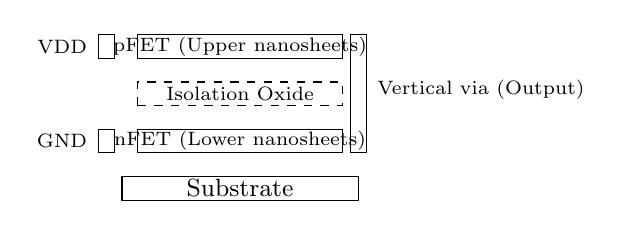
\begin{tikzpicture}[scale=1.0]
% Substrate
\draw (0,0) rectangle (3,0.3);
\node at (1.5,0.15) {\small Substrate};
% nFET
\draw (0.2,0.6) rectangle (2.8,0.9);
\node at (1.5,0.75) {\scriptsize nFET (Lower nanosheets)};
% Isolation oxide
\draw[dashed] (0.2,1.2) rectangle (2.8,1.5);
\node at (1.5,1.35) {\scriptsize Isolation Oxide};
% pFET
\draw (0.2,1.8) rectangle (2.8,2.1);
\node at (1.5,1.95) {\scriptsize pFET (Upper nanosheets)};
% Vias
\draw (2.9,0.6) rectangle (3.1,2.1);
\node[anchor=west] at (3.12,1.4) {\scriptsize Vertical via (Output)};
\draw (-0.3,0.6) rectangle (-0.1,0.9);
\node[anchor=east] at (-0.32,0.75) {\scriptsize GND};
\draw (-0.3,1.8) rectangle (-0.1,2.1);
\node[anchor=east] at (-0.32,1.95) {\scriptsize VDD};
\end{tikzpicture}}
\caption{Sequential CFET cross-section: pFET stacked over nFET with a vertical output via.}
\label{fig:cfet_stack}
\end{figure}

\paragraph*{(ii) Forksheet CFET}
n/p channels are placed orthogonally or laterally separated with a dielectric ``fork'' to ease routing congestion while maintaining strong electrostatics.

\begin{figure}[htbp]
\centering
\fitfig{%
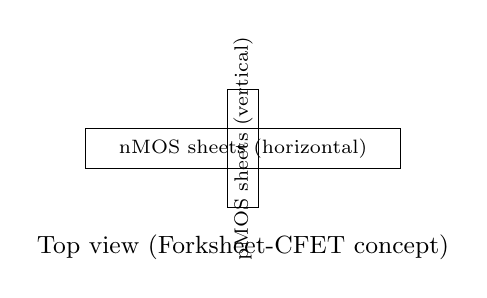
\begin{tikzpicture}[scale=1.0]
% Horizontal nMOS region
\draw (0,0) rectangle (4,0.5);
\node at (2,0.25) {\scriptsize nMOS sheets (horizontal)};
% Vertical pMOS region
\draw (1.8,-0.5) rectangle (2.2,1.0);
\node[rotate=90] at (2.0,0.25) {\scriptsize pMOS sheets (vertical)};
\node at (2,-1.0) {\small Top view (Forksheet-CFET concept)};
\end{tikzpicture}}
\caption{Forksheet-CFET top view concept for routing relief and device isolation.}
\label{fig:forksheet}
\end{figure}

% =========================
\section{Electrical and Layout Impacts}
Key educational points include:
\begin{itemize}
  \item \textbf{Area efficiency:} Sharing lateral footprint across polarities yields near $\sim 2\times$ cell density for inverter-like structures. Benefits propagate to NAND/NOR stacks by co-locating pull-up and pull-down networks.
  \item \textbf{Delay/energy:} The n-to-p connection shortens and becomes a vertical via, reducing local RC. FO1 inverter delay can improve even if single-device $I\!-\!V$ is similar to GAA.
  \item \textbf{Electrostatics:} Each tier can retain GAA-level control; coupling between tiers adds new parasitics (inter-layer capacitance, via resistance).
  \item \textbf{Variability/noise:} Thermal coupling and supply partitioning (VDD up/top, GND down/bottom) introduce asymmetries that must be co-optimized with placement and power routing.
\end{itemize}

% =========================
\section{Manufacturing Challenges}
Independent n/p work-functions and junctions across stacked tiers require selective epitaxy/etch, tight alignment, and low-temperature processes to protect the completed tier.
Dielectric isolation must block dopant/defect diffusion while allowing reliable vertical vias.
BEOL co-design is necessary to partition VDD/GND and to land output vias without penalizing track utilization.

% =========================
\section{Modeling and EDA Limitations}
Compact models publicly available (e.g., BSIM-CMG) capture multi-gate/GAA behavior but not CFET-specific vertical coupling and thermal/variability interactions.
Verilog-A research models exist without consensus, and no open CFET-ready PDKs or standard-cell libraries are available, which itself provides a fertile educational sandbox.\nocite{*}

% =========================
\section{Educational Value}
CFET ties device physics to circuit/layout co-optimization and exposes students to unresolved, multidisciplinary challenges in fabrication, modeling, and CAD---a strong anchor for advanced courses and capstone projects.

% =========================
\section{Conclusion and Outlook}
CFET reframes CMOS as a stacked, cross-sectional inverter.
Beyond electrostatic scaling, it targets wiring delay and footprint.
Research vectors include forksheet layouts, 3D-CFET stacks, thermal-aware power partitioning, and System-on-Stack methodologies.
Embedding CFET in curricula helps prepare engineers for the 2030s.

\section*{Acknowledgment}
The author thanks the Project Design Hub community for discussions.

\bibliographystyle{IEEEtran}
\bibliography{refs}

\section*{Author Biography}
\noindent\textbf{Shinichi Samizo}
received the M.S. degree in Electrical and Electronic Engineering from Shinshu University, Japan.
He worked at Seiko Epson Corporation as an engineer in semiconductor memory and mixed-signal device development, and also contributed to inkjet MEMS actuators and PrecisionCore printhead technology.
He is currently an independent semiconductor researcher focusing on process/device education, memory architecture, and AI system integration.\\[2pt]
\textbf{Contact:} \href{mailto:shin3t72@gmail.com}{shin3t72@gmail.com}, \href{https://github.com/Samizo-AITL}{Samizo-AITL}

\end{document}
